\documentclass{article}
\usepackage[utf8]{inputenc}
\usepackage{amsmath}
\usepackage{listings}
\usepackage{caption}
\usepackage{subcaption}
\usepackage{graphicx}
\usepackage{geometry}

\title{Week 8}
\author{Nicolas Escobar}
\date{\today}

\begin{document}
\maketitle

\section{Bayesian Quantile Regression with BRMS}

Consider the following model:

\begin{align*}
    x \sim \mathrm{Unif} \left(0, 1\right) \\
    y \sim \mathrm{N} \left(0, \exp(2x)\right)
\end{align*}

It is illustrated in Figure \ref{fig:raw}.

\begin{figure}[ht]
    \centering
    
\includegraphics[width=.8\textwidth]{/Users/nescoba/fork_bqsofr/BQSoFR/code_by_nico/memos/data.png}
    \caption{Raw data}
    \label{fig:raw}
\end{figure}

We want to perform Bayesian quantile regression on this data. 
Specifically, we want to model the .25, .5, and .75 quantiles of $y$ as a function of $x$.

The literature would suggest using the following model:

\begin{lstlisting}[language=R]
    GAL2 <- custom_family(
    "GAL2",
    dpars = c("mu", "sigma", "ligam", "tau"), 
    links = c("identity", "log", "identity", "identity"),
    lb = c(NA, 0, Bd[1] * .9, 0), ub = c(NA, NA, Bd[2] * .9, 1), 
    type = "real"
    )
    q25n <- brm(bf(y ~ exp(x), tau = .25), data = synthetic, family = GAL2, 
    stanvars = stanvars2, chains = 2, iter = 2000, control = list(adapt_delta = 0.99), 
    cores = 4, seed = 123)
\end{lstlisting}

However, we suggest modeling the variance separately, as follows:
\begin{lstlisting}
    q25 <- brm(bf(y ~ exp(x), sigma ~ x, tau = .25), data = synthetic, 
    family = GAL2, stanvars = stanvars2, chains = 2, iter = 2000, 
    control = list(adapt_delta = 0.99), cores = 4, seed = 123)
\end{lstlisting}

We found that our suggestion improves the model fit considerably, as illustrated in Figure \ref{fig:q}.

\begin{figure}[ht]
    \centering
    \begin{subfigure}[b]{0.3\textwidth}
        \centering
        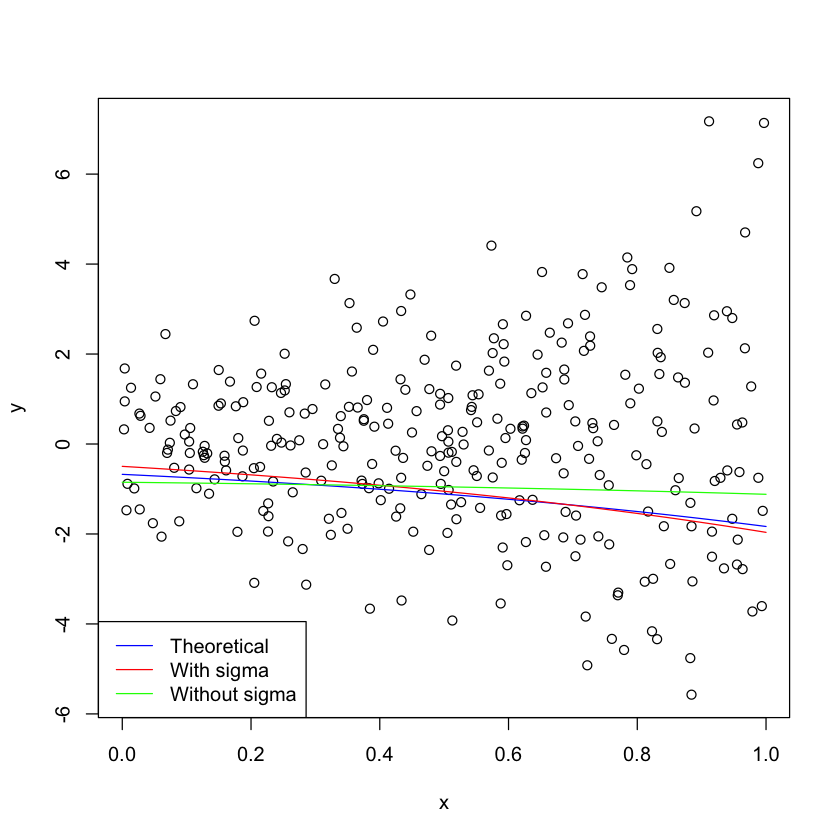
\includegraphics[width=\textwidth]{/Users/nescoba/fork_bqsofr/BQSoFR/code_by_nico/memos/q25.png}
        \caption{.25 Quantile}
    \end{subfigure}
    \hfill
    \begin{subfigure}[b]{0.3\textwidth}
        \centering
        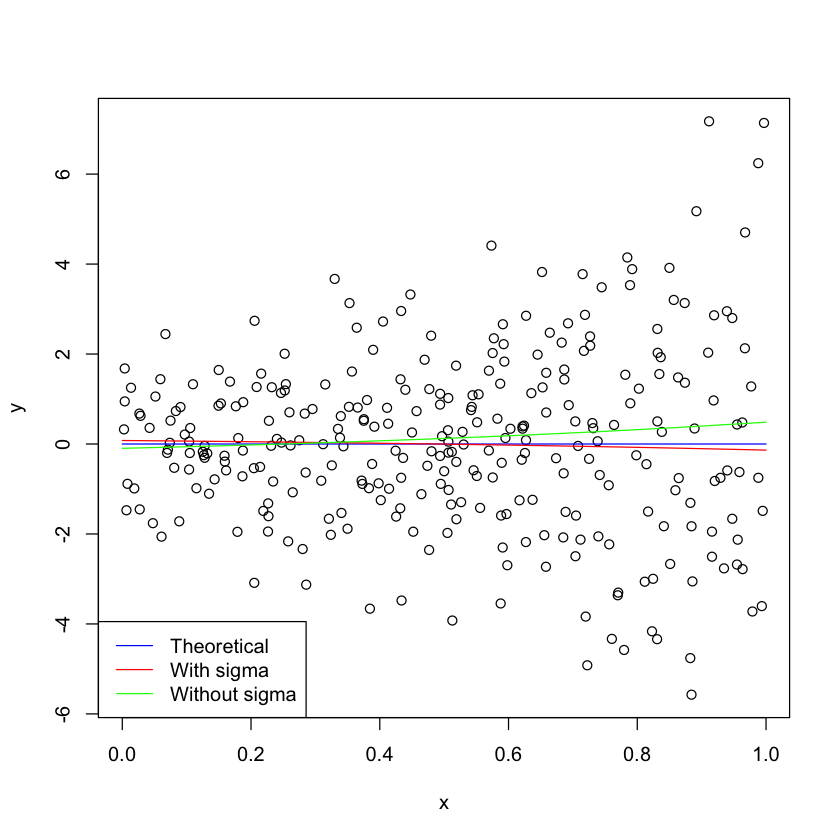
\includegraphics[width=\textwidth]{/Users/nescoba/fork_bqsofr/BQSoFR/code_by_nico/memos/q50.png}
        \caption{.5 Quantile}
    \end{subfigure}
    \hfill
    \begin{subfigure}[b]{0.3\textwidth}
        \centering
        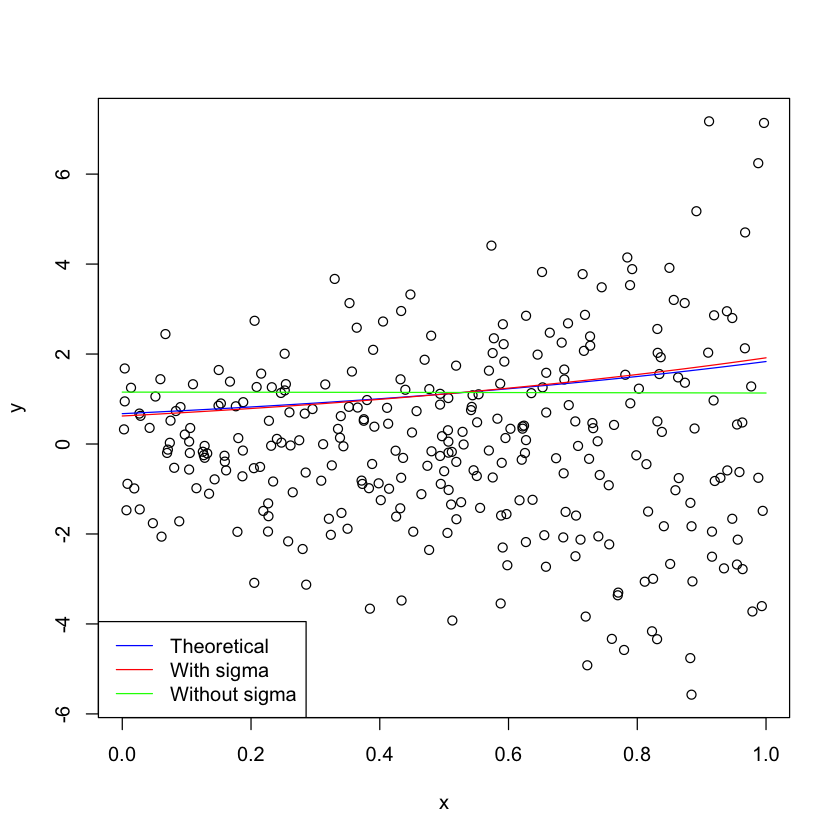
\includegraphics[width=\textwidth]{/Users/nescoba/fork_bqsofr/BQSoFR/code_by_nico/memos/q75.png}
        \caption{.75 Quantile}
    \end{subfigure}
    \caption{Quantile Regression}
    \label{fig:q}
\end{figure}

In the previous models, we told \texttt{brms} explicitely that the location parameter
was an exponential function of $x$. We further explored this avenue and told \texttt{brms} 
only that the location parameter was a smooth function of $x$:

\begin{lstlisting}[language=R]
    q25 <- brm(bf(y ~ s(x), sigma ~ x, tau = .25), data = synthetic, 
    family = GAL2, stanvars = stanvars2, chains = 2, iter = 2000, 
    control = list(adapt_delta = 0.99), cores = 4, seed = 123)
\end{lstlisting}

BRMS was able to recover the appropriate shape of the location parameter, as illustrated in Figure \ref{fig:q25}.

\begin{figure}[ht]
    \centering
    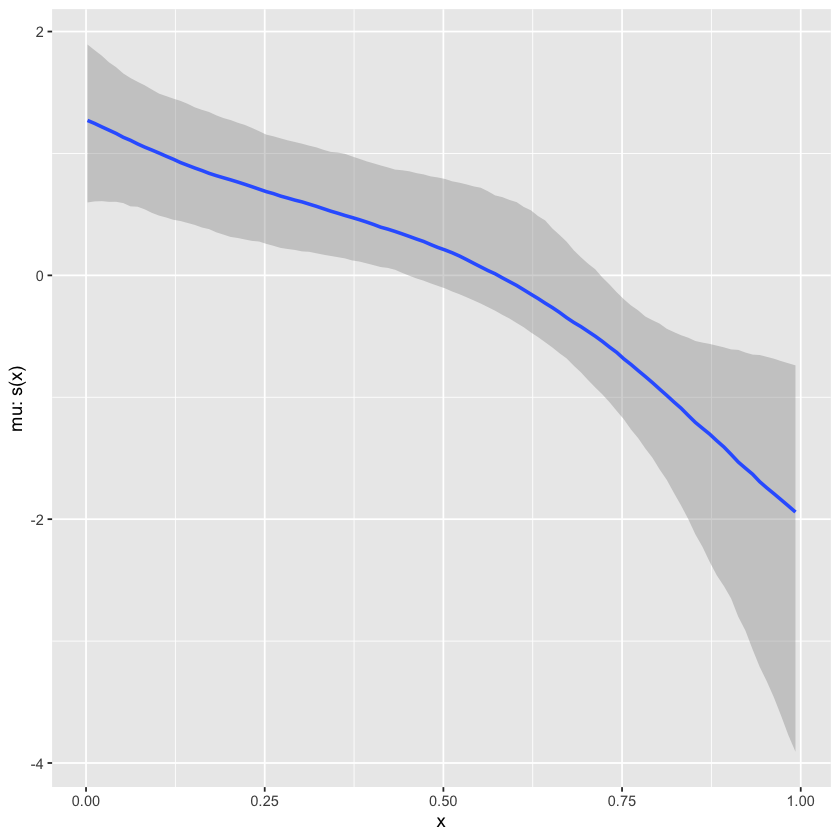
\includegraphics[width=.8\textwidth]{/Users/nescoba/fork_bqsofr/BQSoFR/code_by_nico/memos/q25s.png}
    \caption{.25 Quantile}
    \label{fig:q25}
\end{figure}

\section{Latent Factor Models}

Consider the following model in \texttt{lavaan} syntax:

\begin{lstlisting}[language=R]
    mod <- 
    "
    f2 =~ x01 + x02
    x03 ~ f2
    "
    fit_lavaan <- sem(mod, data = dat)
\end{lstlisting}

We would like to fit this model with \texttt{brms}. 
This is not possible with the current version of \texttt{brms}, but we can use the following workaround:

\begin{lstlisting}[language=R]
    # Creating empty column for the mediator
    dat$f1 <- as.numeric(NA)

    # Defining the dependency of the mediator on observed variables: 
    bf1 <- bf(x01 ~ 0 + mi(f1))
    bf2 <- bf(x02 ~ 0 + mi(f1))

    # Telling brms that the mediator is a latent variable
    bf3 <- bf(f1 | mi() ~ 0)

    # Defining the dependency of the outcome on the mediator
    bf4 <- bf(x03 ~ 0 + mi(f1))

    # Fitting the brms object 
    fit_brms <- brm(bf1 + bf2 + bf3 + bf4 + set_rescor(FALSE), data = dat, 
    iter = 2000, chains = 2, cores = 4, seed = 123, prior = prior(normal(1, 0.00001), 
    coef = mif1, resp = x01))
\end{lstlisting}

The coefficients obtained this way are similar to the ones obtained with \texttt{lavaan}.

\section{R Package}

I started working on the R package for the grant. 
I will be working on the Corrected Score paper. 
I took a preliminary look at the code and refreshed my memory about how to write packages in R.


\end{document}
